\section{Parte 2: Sesión de Planning Poker}

\subsection{Dinámica de la Sesión en el Laboratorio}

La sesión de Planning Poker se llevó a cabo de manera presencial entre los tres integrantes del equipo de desarrollo: \textbf{Noe Franklin Choquenaira Quispe}, \textbf{Aldo Yaranga Achahui} y \textbf{Carolay Ccama Enriquez}. Para garantizar el rigor metodológico exigido por la guía de laboratorio, se siguió estrictamente el protocolo de cinco pasos para cada una de las 13 historias de usuario:

\begin{enumerate}
    \item \textbf{Selección y lectura de la historia:} Siguiendo el orden de prioridad MoSCoW, se leyó en voz alta la historia de usuario junto con sus criterios de aceptación. El Product Owner aclaró el alcance funcional esperado.
    \item \textbf{Asignación secreta del valor:} Cada integrante seleccionó en privado su estimación en la baraja digital de Fibonacci ($1, 2, 3, 5, 8, 13, 21$), evaluando mentalmente el esfuerzo, la complejidad algorítmica y la incertidumbre técnica frente a la historia de referencia (\texttt{HU-12} = 3 SP).
    \item \textbf{Revelación simultánea y comparación:} A la cuenta de tres, todos los integrantes revelaron sus cartas al unísono. Si los valores coincidían plenamente o distaban en solo un peldaño contiguo de la escala, se procedía a un ajuste rápido.
    \item \textbf{Discusión técnica de discrepancias:} Cuando la distancia entre votos era de dos o más posiciones en la escala Fibonacci, se abrió de inmediato el debate. El participante con el voto más alto explicó los riesgos o dificultades técnicas que vislumbraba, mientras que el participante con el voto más bajo argumentó por qué consideraba la tarea más sencilla o reutilizable.
    \item \textbf{Consenso y segunda ronda:} Tras la deliberación, se realizó una segunda ronda de votación para las historias polémicas o se formalizó el consenso unánime del valor final.
\end{enumerate}

La Figura~\ref{fig:sesion_planning_poker} exhibe el panel digital de la sesión, donde se aprecian las tarjetas con los votos individuales por ronda de cada integrante (resaltando en rojo el voto más alto y en verde el voto más bajo) y el puntaje final de consenso.

\begin{figure}[H]
    \centering
    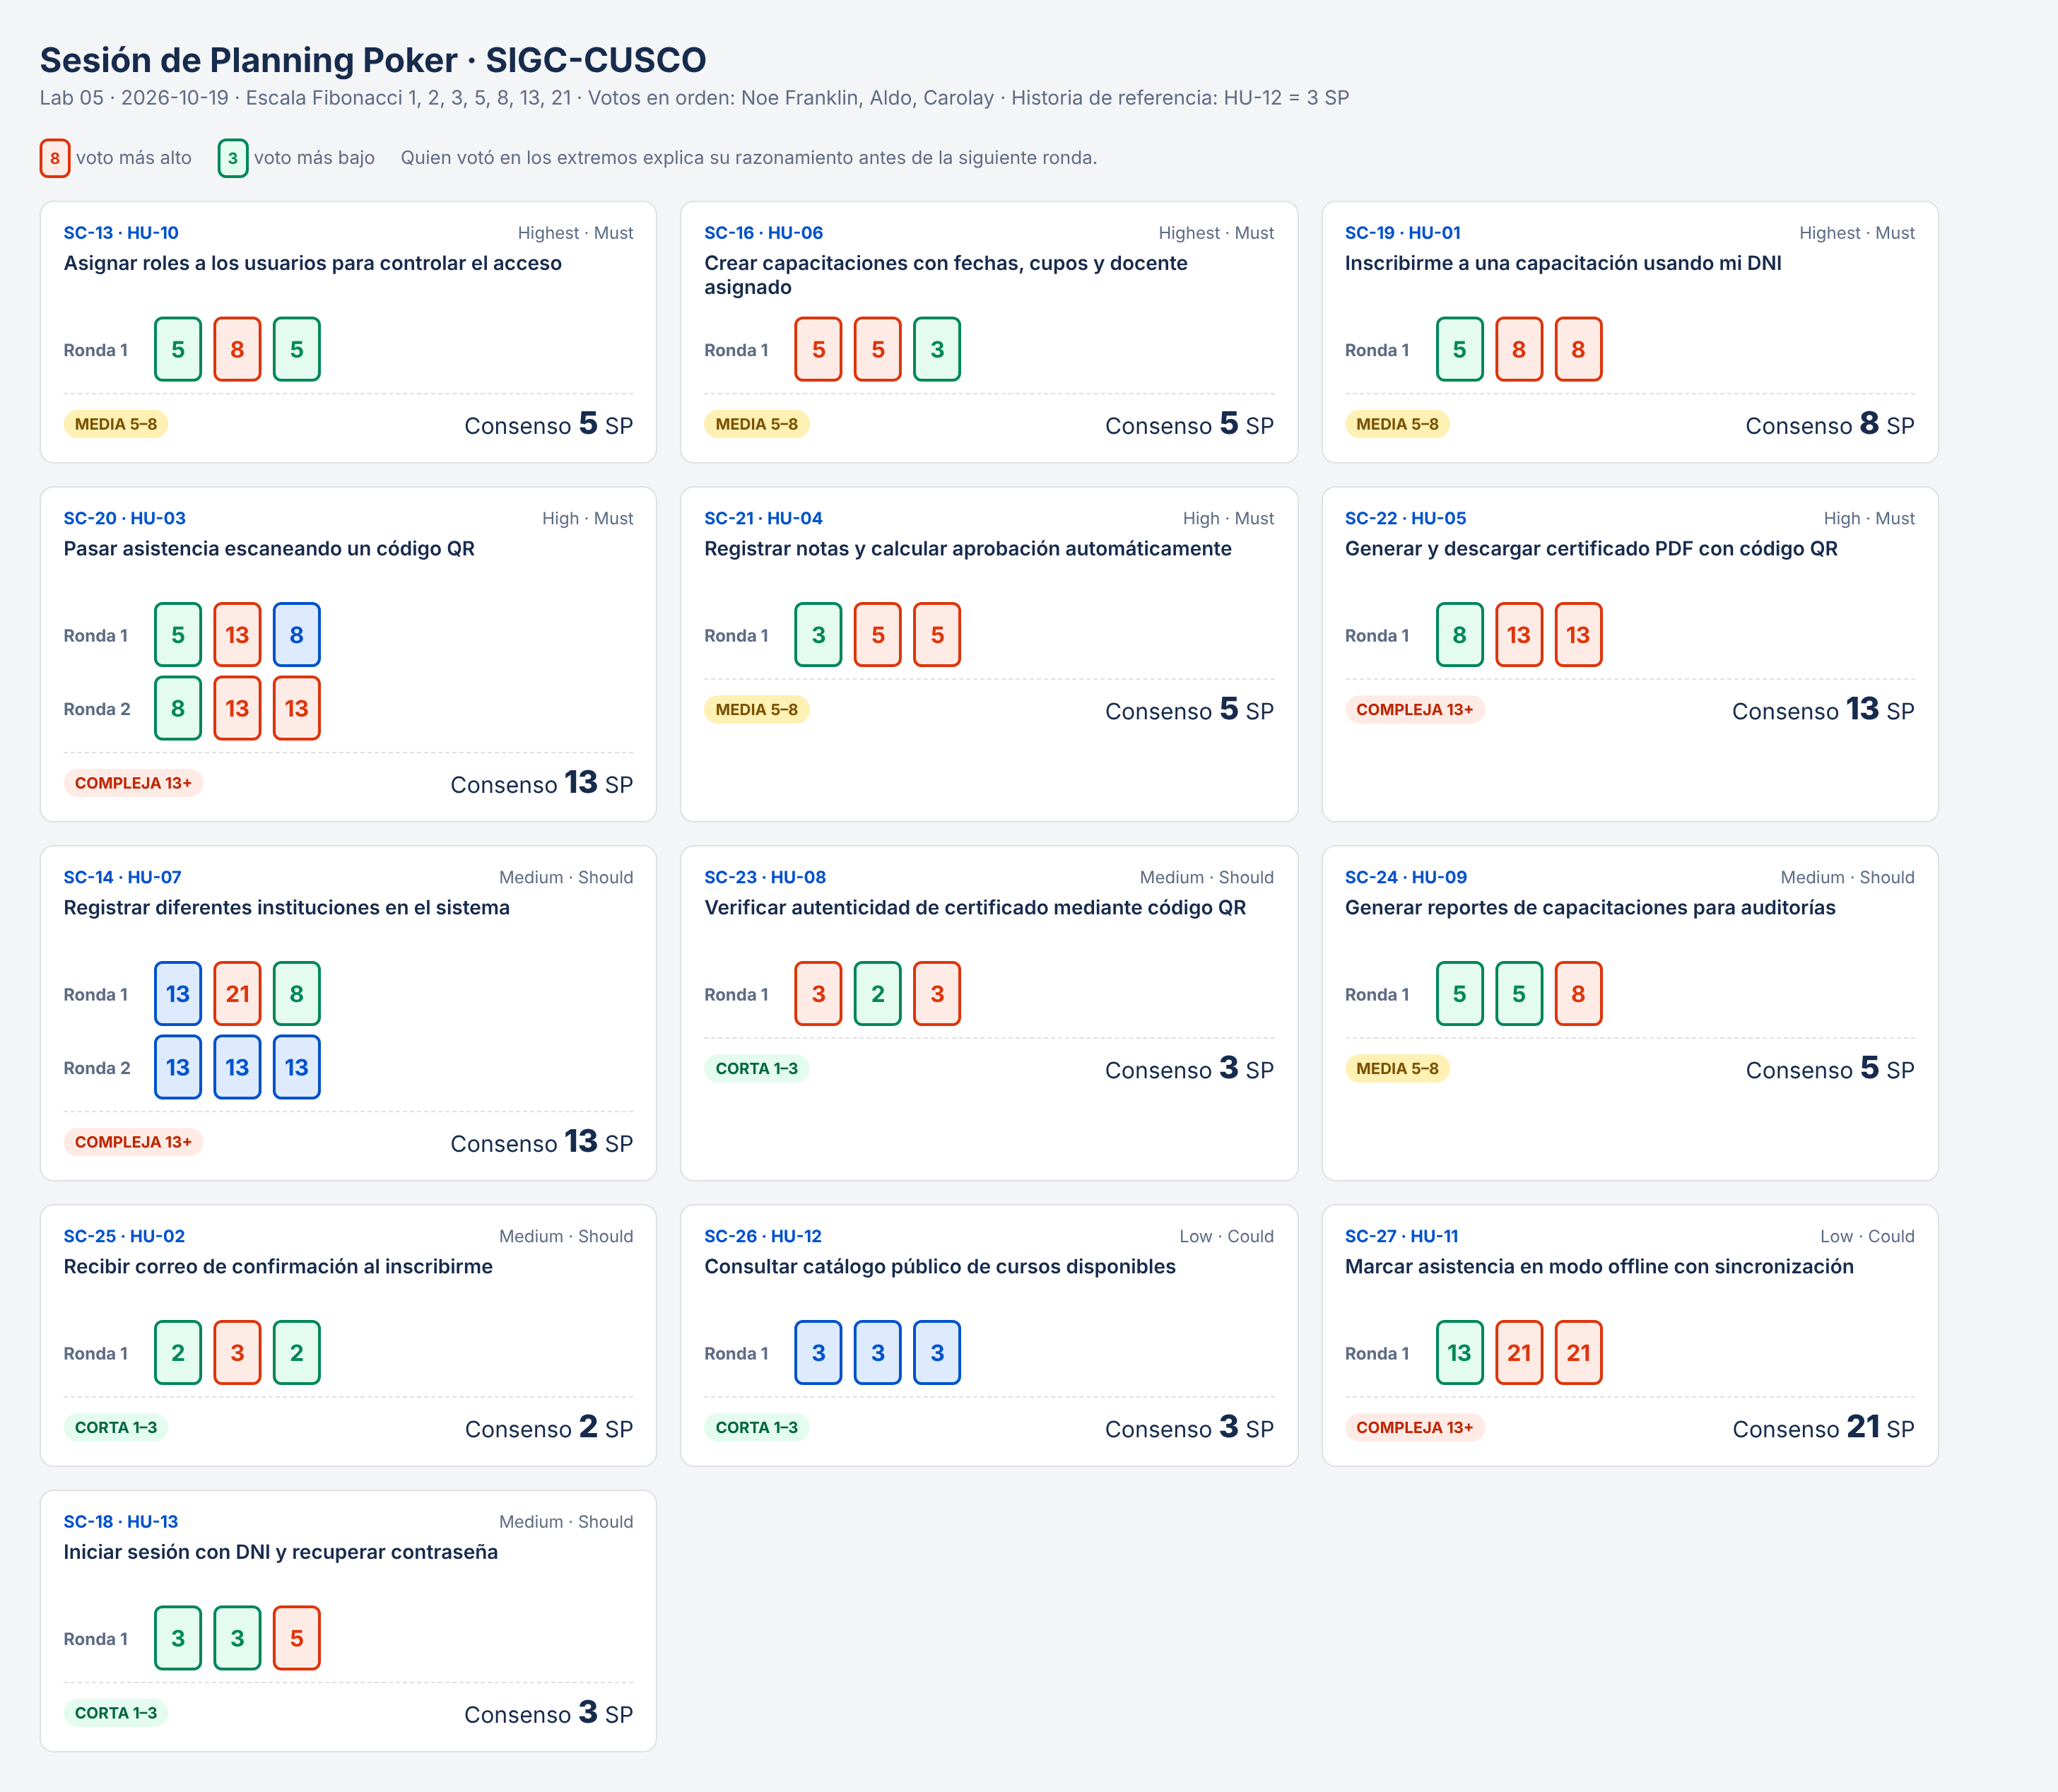
\includegraphics[width=\textwidth]{figura1_sesion_planning_poker.png}
    \caption{Evidencia gráfica de la sesión de Planning Poker: votos individuales por ronda de los tres integrantes y valor de consenso acordado por historia (rojo = voto más alto, verde = voto más bajo).}
    \label{fig:sesion_planning_poker}
\end{figure}

\subsection{Votos por Historia y Rondas de Deliberación}

En la Tabla~\ref{tab:votos_sesion} se registra el historial de votaciones obtenido durante la dinámica, mostrando las estimaciones de cada integrante en el orden cronológico de votación: \textbf{Noe Franklin / Aldo / Carolay}.

\begin{table}[H]
\centering
\small
\renewcommand{\arraystretch}{1.2}
\caption{Registro de votos individuales por ronda y consenso alcanzado (orden: Noe Franklin / Aldo / Carolay).}
\label{tab:votos_sesion}
\begin{tabularx}{\textwidth}{P{1.4cm} P{1.4cm} Y P{3.2cm} C{1.8cm}}
\toprule
\rowcolor{headerblue}
\textcolor{white}{\textbf{Clave}} & \textcolor{white}{\textbf{Código}} & \textcolor{white}{\textbf{Historia de Usuario}} & \textcolor{white}{\textbf{Votos por Ronda}} & \textcolor{white}{\textbf{Consenso SP}} \\
\midrule
\rowcolor{white}
SC-13 & HU-10 & Asignar roles a los usuarios para controlar el acceso & R1: 5 / 8 / 5 & \textbf{5 SP} \\
\rowcolor{rowalt}
SC-16 & HU-06 & Crear capacitaciones con fechas, cupos y docente asignado & R1: 5 / 5 / 3 & \textbf{5 SP} \\
\rowcolor{white}
SC-19 & HU-01 & Inscribirme a una capacitación usando mi DNI & R1: 5 / 8 / 8 & \textbf{8 SP} \\
\rowcolor{rowalt}
SC-20 & HU-03 & Pasar asistencia escaneando un código QR & R1: 5 / 13 / 8 \newline R2: 8 / 13 / 13 & \textbf{13 SP} \\
\rowcolor{white}
SC-21 & HU-04 & Registrar notas y calcular aprobación automáticamente & R1: 3 / 5 / 5 & \textbf{5 SP} \\
\rowcolor{rowalt}
SC-22 & HU-05 & Generar y descargar certificado PDF con código QR & R1: 8 / 13 / 13 & \textbf{13 SP} \\
\rowcolor{white}
SC-14 & HU-07 & Registrar diferentes instituciones en el sistema & R1: 13 / 21 / 8 \newline R2: 13 / 13 / 13 & \textbf{13 SP} \\
\rowcolor{rowalt}
SC-23 & HU-08 & Verificar autenticidad de certificado mediante código QR & R1: 3 / 2 / 3 & \textbf{3 SP} \\
\rowcolor{white}
SC-24 & HU-09 & Generar reportes de capacitaciones para auditorías & R1: 5 / 5 / 8 & \textbf{5 SP} \\
\rowcolor{rowalt}
SC-25 & HU-02 & Recibir correo de confirmación al inscribirme & R1: 2 / 3 / 2 & \textbf{2 SP} \\
\rowcolor{white}
SC-26 & HU-12 & Consultar catálogo público de cursos disponibles & R1: 3 / 3 / 3 & \textbf{3 SP} \textit{(Ref.)} \\
\rowcolor{rowalt}
SC-27 & HU-11 & Marcar asistencia en modo offline con sincronización & R1: 13 / 21 / 21 & \textbf{21 SP} \\
\rowcolor{white}
SC-18 & HU-13 & Iniciar sesión con DNI y recuperar contraseña & R1: 3 / 3 / 5 & \textbf{3 SP} \\
\bottomrule
\end{tabularx}
\end{table}

\subsection{Discusión Técnica y Argumentación del Consenso}

A continuación, se documenta la deliberación técnica suscitada en cada una de las historias de usuario, reflejando los motivos que llevaron al equipo a converger en el valor de consenso:

\begin{itemize}
    \item \textbf{HU-10: Asignar roles a los usuarios (5 SP):} En la primera ronda, Aldo votó \textbf{8} al considerar que se debía diseñar un esquema dinámico de permisos modulares granulares (matriz RBAC configurable en base de datos tipo paquete Spatie). Franklin y Carolay (ambos con voto \textbf{5}) argumentaron que el alcance para esta versión del SIGC-CUSCO requiere únicamente cuatro roles predefinidos (\textit{SuperAdmin}, \textit{Admin Entidad}, \textit{Docente} y \textit{Participante}), implementables de manera limpia mediante \textit{Gates} y \textit{Policies} nativas de Laravel. Aldo coincidió en que restringir los roles a un conjunto fijo disminuye drásticamente el esfuerzo, consolidándose el consenso en \textbf{5 SP}.
    
    \item \textbf{HU-06: Crear capacitaciones con fechas y cupos (5 SP):} Carolay emitió un voto de \textbf{3}, concibiéndola como un formulario CRUD estándar sobre la tabla de cursos. Franklin y Aldo (ambos con \textbf{5}) le hicieron notar la lógica de negocio subyacente: validación de coherencia temporal (fecha de inicio anterior a fin, fecha límite de inscripción), cruce de horarios para que un docente no sea asignado a dos capacitaciones simultáneas, y la transición automática de estados del curso (\textit{Borrador}, \textit{Abierto}, \textit{En Curso}, \textit{Finalizado}). Carolay reconoció estas restricciones de integridad y se convino \textbf{5 SP}.
    
    \item \textbf{HU-01: Inscribirme a una capacitación usando DNI (8 SP):} Franklin votó \textbf{5}, pensando únicamente en la captura del formulario de inscripción. Por el contrario, Aldo y Carolay votaron \textbf{8} señalando dos riesgos mayúsculos: la necesidad de validar el formato y dígito verificador del DNI peruano (o consumir un servicio REST de RENIEC con control de timeouts/caché) y, primordialmente, el control de concurrencia en la asignación de cupos. Para evitar sobrecupos (\textit{race conditions}) cuando varios postulantes se inscriben al mismo segundo para la última vacante, se requiere el uso de transacciones atómicas de base de datos (\texttt{DB::transaction}) con bloqueo pesimista (\texttt{lockForUpdate}). Franklin aceptó la trascendencia técnica de este riesgo y se consensuó en \textbf{8 SP}.
    
    \item \textbf{HU-03: Pasar asistencia escaneando código QR (13 SP):} Esta historia generó la mayor dispersión inicial de la jornada: Franklin votó \textbf{5}, Carolay \textbf{8} y Aldo \textbf{13}. Franklin propuso una solución elemental: proyectar un código QR estático en la pizarra del aula para que los alumnos lo escanearan con el celular. Aldo refutó inmediatamente esta idea, demostrando que un QR estático es vulnerable al fraude académico: un estudiante en el aula puede fotografiar el QR y enviarlo vía WhatsApp a compañeros ausentes para que marquen asistencia desde sus casas. Para cumplir los estándares de seguridad, el sistema debe generar un QR dinámico con token criptográfico temporal (TOTP) que expire cada 20 a 30 segundos, validando además que un participante no registre dos veces su asistencia en la misma sesión. Carolay respaldó la necesidad de robustez y, en la segunda ronda, los votos fueron \textbf{8 / 13 / 13}, acordando unánimemente \textbf{13 SP}. Por su tamaño y riesgo, fue clasificada como candidata prioritaria para refinamiento.
    
    \item \textbf{HU-04: Registrar notas y calcular aprobación automáticamente (5 SP):} Franklin votó \textbf{3}, mientras que Aldo y Carolay votaron \textbf{5}. La regla de negocio base (nota final $\ge 11$ en la escala vigesimal de 0 a 20) es sencilla; no obstante, el flujo exige una matriz interactiva de calificaciones para el docente, validación estricta de rangos y el mecanismo formal de \enquote{Cierre de Acta}, el cual debe sellar la edición de notas de manera irreversible para garantizar la inmutabilidad de los registros académicos. El equipo acordó rápidamente fijar la historia en \textbf{5 SP}.
    
    \item \textbf{HU-05: Generar y descargar certificado PDF con código QR (13 SP):} Votada con \textbf{8 / 13 / 13}. Franklin pensó que la librería \texttt{DomPDF} simplificaría todo el proceso; sin embargo, Aldo y Carolay explicaron la amplitud del alcance: se debe verificar que el alumno cumpla doble condición (nota aprobatoria $\ge 11$ y asistencia mínima al $80\%$), diseñar la maqueta visual del diploma con tipografía y escudo institucional, calcular un hash SHA-256 único antifalsificación incrustado en el documento, generar un código QR vectorial de validación y proveer la capacidad de descarga masiva para el docente. Ante la envergadura del motor de generación, Franklin aceptó el consenso en \textbf{13 SP}, programándose su refinamiento en historias más pequeñas.
    
    \item \textbf{HU-07: Registrar diferentes instituciones en el sistema (13 SP):} La primera ronda mostró una discordancia crítica: Franklin votó \textbf{13}, Aldo \textbf{21} y Carolay \textbf{8}. Carolay consideraba únicamente la interfaz administrativa para dar de alta una institución (RUC, nombre, logo). Por su parte, Aldo contemplaba el peor escenario de la arquitectura multientidad: separar los datos en esquemas o bases de datos físicas independientes, lo cual disparaba el esfuerzo a 21 SP. En la discusión se clarificó la decisión de diseño: se empleará un esquema compartido con clave foránea \texttt{institution\_id} y \textit{Global Scopes} de Eloquent en Laravel para filtrar automáticamente los registros. Esta aclaración disipó el temor de bases de datos aisladas pero mantuvo la necesidad de auditar que ningún controlador filtre información entre entidades. En la segunda ronda, la votación fue unánime: \textbf{13 / 13 / 13} (\textbf{13 SP}).
    
    \item \textbf{HU-08: Verificar autenticidad de certificado mediante QR (3 SP):} Votación expedita (Franklin \textbf{3}, Aldo \textbf{2}, Carolay \textbf{3}). Consiste en un endpoint público de solo lectura que recibe el hash o código del certificado y devuelve el estado de validez institucional. Al depender del esquema ya resuelto en \texttt{HU-05}, su complejidad es mínima. Consenso cerrado en \textbf{3 SP}.
    
    \item \textbf{HU-09: Generar reportes para auditorías (5 SP):} Carolay votó \textbf{8} anticipando exigencias complejas de auditoría gubernamental (OSCE / Contraloría). Tras deliberar, el equipo acordó estructurar una plantilla consolidada estándar en formato Excel (.xlsx) mediante la librería \texttt{PhpSpreadsheet}, con totales de inscritos, asistencias y notas. Se cerró en \textbf{5 SP}.
    
    \item \textbf{HU-02: Correo de confirmación de inscripción (2 SP):} Votación baja (Franklin \textbf{2}, Aldo \textbf{3}, Carolay \textbf{2}). El framework Laravel ya cuenta con el sistema de mensajería asíncrona (\texttt{Mailable}) y colas de trabajo (\textit{Queues}) preconfigurado; únicamente se requiere maquetar la plantilla HTML responsiva y disparar el evento tras la persistencia de la inscripción. Consenso en \textbf{2 SP}.
    
    \item \textbf{HU-12: Catálogo público de cursos (3 SP):} Historia de referencia del equipo. La votación fue unánime en primera ronda (\textbf{3 / 3 / 3}).
    
    \item \textbf{HU-11: Marcar asistencia en modo offline con sincronización (21 SP):} Votación contundente: Franklin \textbf{13}, Aldo \textbf{21} y Carolay \textbf{21}. Constituye la funcionalidad de mayor incertidumbre técnica de todo el SIGC-CUSCO. El requerimiento exige que los docentes en zonas rurales de la región Cusco (sin cobertura de internet) puedan pasar asistencia en sus dispositivos móviles y que, al recuperar la conexión, las asistencias se sincronicen bidireccionalmente sin generar duplicados ni sobrescribir registros previos. Dado que ningún integrante del equipo ha implementado previamente \textit{Service Workers}, almacenamiento en \textit{IndexedDB} y protocolos de resolución de conflictos, la incertidumbre es máxima. El equipo acordó unánimemente el techo de la escala: \textbf{21 SP}, determinando que es mandatorio aislar la tecnología mediante un spike de investigación en el trabajo extra.
    
    \item \textbf{HU-13: Iniciar sesión con DNI y recuperar contraseña (3 SP):} Votos \textbf{3 / 3 / 5}. Carolay votó 5 previendo el flujo de tokens por correo; no obstante, el kit de autenticación de Laravel resuelve nativamente el hashing de contraseñas con Bcrypt, la expiración de enlaces y las sesiones seguras, requiriendo únicamente cambiar la columna de autenticación de \texttt{email} a \texttt{dni}. Consenso en \textbf{3 SP}.
\end{itemize}

\subsection{Análisis de Dispersión y Comportamiento del Consenso}

Al analizar estadísticamente los resultados de la sesión, se constata que:
\begin{enumerate}
    \item En \textbf{10 de las 13 historias} (el $77\%$), el equipo alcanzó consenso en la primera ronda con diferencias máximas de un peldaño contiguo en Fibonacci, evidenciando un entendimiento alineado del alcance general del sistema.
    \item Únicamente en \textbf{3 historias} (\texttt{HU-03}, \texttt{HU-07} y \texttt{HU-11}) se registraron divergencias profundas ($\ge 2$ niveles de la escala). Resulta sumamente significativo que estas tres historias coincidieran con las funcionalidades de mayor incertidumbre técnica y riesgos de arquitectura (prevención de fraude en QR, aislamiento multientidad y persistencia offline).
    \item El ejercicio demostró el valor cardinal del Planning Poker: la revelación simultánea desarticuló cualquier sesgo de anclaje, y los debates técnicos sacaron a flote requisitos no funcionales críticos (concurrencia, seguridad criptográfica y manejo de estados sin red) que habrían pasado desapercibidos en una estimación individual.
\end{enumerate}
